
\chapter{អ៊ីពែបូល}
\section{សញ្ញាណអ៊ីពែបូល}
%
\begin{definition*}
	\emph{អ៊ីពែបូល} ជាសំណុំចំណុចក្នុងប្លង់ដែលមានគម្លាតរវាងចម្ងាយពីចំណុចនោះទៅចំណុចនឹងពីរជាចំនួនថេរ។
\end{definition*}
\begin{figure}[H]
	\centering
	\caption{អ៊ីពែបូល}
	\begin{tikzpicture}[x=.25cm,y=.25cm,every node/.style={font=\scriptsize,text=magenta}]
		\coordinate(X')at(-14,0);
		\coordinate(X)at(14,0);
		\coordinate(Y')at(0,-10);
		\coordinate(Y)at(0,10);
		\coordinate(F1)at(-5,0);
		\coordinate(F2)at(5,0);
		\coordinate(V1)at(-4,0);
		\coordinate(V2)at(4,0);
		\coordinate(I)at(0,0);
		\coordinate(Q)at(8,5.2);
		\draw[dotted](X')--node[sloped,very near end,above]{អ័ក្សទទឹង}(X);
		\draw[dotted](Y')--node[sloped,very near end,above]{អ័ក្សឆ្លុះ}(Y);
		\draw([yshift=1ex]I)--([xshift=1ex,yshift=1ex]I)--([xshift=1ex]I);
		\draw[magenta,samples=50,domain=-0.74:0.74] plot ({4.*(1+(\x)^2)/(1-(\x)^2)},{3.*2*(\x)/(1-(\x)^2)});
		\draw[magenta,samples=50,domain=-0.74:0.74] plot ({4.*(-1-(\x)^2)/(1-(\x)^2)},{3.*(-2)*(\x)/(1-(\x)^2)});
		\draw(F1)node[left]{$ F_1 $}--node[sloped,above]{$ d_1 $}(Q)node[above]{$ Q $}--node[sloped,below]{$ d_2 $}(F2)node[right]{$ F_2 $};
		\foreach\p in{F1,F2,V1,V2,Q}{\fill[red](\p)circle(1.5pt);}
		\node[text=blue]at(0,-5){$ |d_1-d_2|=\text{ចំនួនថេរ} $};
		\node[below left]at(O){$ O $};
		\node[right]at(V1){$ V_1 $};
		\node[left]at(V2){$ V_2 $};
	\end{tikzpicture}
\end{figure}
%
\begin{itemize}
	\item ចំណុចនឹងទាំងពីរហៅថា \emph{កំណុំ} តាងដោយ $ F_1 $ និង $ F_2 $
	\item ចំណុចកណ្ដាលរវាងកំណុំទាំងពីរហៅថា \emph{ផ្ចិត} តាងដោយ $ I $
	\item ចម្ងាយរវាងកំណុំទាំងពីរតាងដោយ $ F_1F_2=2c $
	\item ប្រសព្វរវាងអង្កត់ $ [F_1F_2] $ និង អ៊ីពែបូលហៅថា \emph{កំពូល} តាងដោយ $ V_1 $ និង $ V_2 $
	\item ចម្ងាយរវាងកំពូលទាំងពីរតាងដោយ $ V_1V_2=2a $
	\item បន្ទាត់ដែលកាត់តាមកំណុំទាំងពីរហៅថា \emph{អ័ក្សទទឹង}% តាងដោយ
	\item មេដ្យ៉ាទ័រនៃអង្កត់ $ [F_1F_2] $ ហៅថា \emph{អ័ក្សឆ្លុះ}
\end{itemize}
%
\section{សមីការស្តង់ដានៃអ៊ីពែបូល}
\subsection{អ័ក្សទទឹងស្របអ័ក្សអាប់ស៊ីស}
\begin{proposition*}
	អ៊ីពែបូល $ (H) $ ដែលមានអ័ក្សទទឹងស្របអ័ក្សអាប់ស៊ីសនិងមាន
	\begin{itemize}
		\item ផ្ចិត $ I(h,k) $
		\item កំពូល $ V_1(h-a,k) $ និង $ V_2(h+a,k) $
		\item កំណុំ $ F_1(h-c,k) $ និង $ F_2(h+c,k) $
	\end{itemize}
	មានសមីការស្តង់ដា
	\begin{equation}
		(H):\dfrac{(x-h)^2}{a^2}-\dfrac{(y-k)^2}{b^2}=1\quad\text{ដែល}\;b^2=c^2-a^2
	\end{equation}
	ហើយមានអាស៊ីមតូត
	\begin{itemize}[2]
		\item $ \dfrac{x-h}{a}-\dfrac{y-k}{b}=0 $
		\item $ \dfrac{x-h}{a}+\dfrac{y-k}{b}=0 $~។
	\end{itemize}
\end{proposition*}
%
\begin{figure}[H]
	\centering
	\begin{tikzpicture}[x=.5cm,y=.5cm,every node/.style={font=\scriptsize,text=magenta}]
		\coordinate(O)at(0,0);
		\coordinate(X')at(-4,0);
		\coordinate(X)at(6,0);
		\coordinate(Y')at(0,-4);
		\coordinate(Y)at(0,8);
		\coordinate(I)at(1,2);
		\coordinate(V1)at(-1,2);
		\coordinate(V2)at(3,2);
		\coordinate(F1)at(-2.61,2);
		\coordinate(F2)at(4.61,2);
		\coordinate(Q)at(4,5.35);
		\coordinate(R)at(0,-2);
		\coordinate(S)at(0,-3);
		%c: (x - 1)² / 2² - (y - 2)² / 3² = 1
		\draw[->](X')node[left]{$ x' $}--(X)node[right]{$ x $};
		\draw[->](Y')node[below]{$ y' $}--(Y)node[above]{$ y $};
		\draw[dashed](F1-|X')--(F2-|X);
		\draw[magenta]plot[samples=50,domain=-0.618:0.618]({2*(1+\x*\x)/(1-\x*\x)+1},{3*(2*\x)/(1-\x*\x)+2});
		\draw[magenta]plot[samples=50,domain=-0.618:0.618]({2*(1+\x*\x)/(-1+\x*\x)+1},{3*(2*\x)/(-1+\x*\x)+2});
		\draw(F1)--(Q)--(F2);
		\foreach\p in{V1,V2}{\draw[dashed](\p)--(\p|-R);}
		\draw[<->](V1|-R)--node[above]{$ a $}(I|-R);
		\draw[<->](I|-R)--node[above]{$ a $}(V2|-R);
		\foreach\p in{F1,F2,I}{\draw[dashed](\p)--(\p|-S);}
		\draw[<->](F1|-S)--node[below]{$ c $}(I|-S);
		\draw[<->](I|-S)--node[below]{$ c $}(F2|-S);
		\foreach\p in{I,V1,V2,F1,F2,Q}{\fill[red](\p)circle(1.5pt);}
		\node[above]at(I){$ I $};
		\node[above left]at(F1){$ F_1 $};
		\node[above right]at(F2){$ F_2 $};
		\node[above right]at(V1){$ V_1 $};
		\node[above left]at(V2){$ V_2 $};
		\node[above left]at(Q){$ Q $};
		\node[below right]at(I|-X){$ h $};
		\node[above right]at(I-|Y){$ k $};
		\node[above right,text=blue](axis)at(-4,4){អ័ក្សទទឹង};
		\draw[->](-4,2)to[out=90,in=270](axis);
	\end{tikzpicture}
\end{figure}
%
\begin{example*}
	សរសេរសមីការស្តង់ដានៃអ៊ីពែបូលដែលមានផ្ចិត $ I(0,0) $ កំពូល $ V_2(4,0) $ និងកំណុំ $ F_2(5,0) $~។
\end{example*}
%
\begin{answer}
	តាមសម្មតិកម្មយើងបាន
	\begin{itemize}
		\item $ I(0,0) $ នោះ $ h=0 $ និង $ k=0 $
		\item កន្លះចម្ងាយរវាងកំពូល $ a=IV_2=\sqrt{(4-0)^2+(0-0)^2}=4 $
		\item កន្លះចម្ងាយរវាងកំណុំ $ c=IF_2=\sqrt{(5-0)^2+(0-0)^2}=5 $
		\item នោះ $ b=\sqrt{c^2-a^2}=\sqrt{5^2-4^2}=3 $
	\end{itemize}
	ដោយអរដោនេនៃផ្ចិត កំពូល កំណុំ ស្មើ $ 0 $ ដូចគ្នានោះអ៊ីពែបូលមានអ័ក្សទទឹងស្របអ័ក្សអាប់ស៊ីស នាំឲ្យសមីការស្តង់ដាអ៊ីពែបូលមានទម្រង់\\ $ \dfrac{(x-h)^2}{a^2}-\dfrac{(y-k)^2}{b^2}=1 $~។\\ ដូច្នេះ អ៊ីពែបូលមានសមីការស្តង់ដា $ \dfrac{(x-0)^2}{4^2}-\dfrac{(y-0)^2}{3^2}=1 $~។
\end{answer}
%
\begin{example*}
	សរសេរសមីការស្តង់ដានៃអ៊ីពែបូលដែលមានផ្ចិត $ (1,2) $ កំពូល $ (4,2) $ និងកំណុំ $ (-4,2) $~។
\end{example*}
%
\begin{answer}
	តាមសម្មតិកម្មយើងបាន
	\begin{itemize}
		\item កំពូល $ (1,2) $ នោះ $ h=1 $ និង $ k=2 $
		\item ចម្ងាយពីផ្ចិតទៅកំពូល $ a=\sqrt{(4-1)^2+(2-2)^2}=3 $
		\item ចម្ងាយពីផ្ចិតទៅកំណុំ $ c=\sqrt{(-4-1)^2+(2-2)^2}=5 $
		\item នោះ $ b=\sqrt{c^2-a^2}=\sqrt{5^2-3^2}=4 $
	\end{itemize}
	ដោយអរដោនេនៃផ្ចិត កំពូល កំណុំ ស្មើ $ 2 $ ដូចគ្នានោះអ៊ីពែបូលមានអ័ក្សទទឹងស្របអ័ក្សអាប់ស៊ីស នាំឲ្យសមីការស្តង់ដាអ៊ីពែបូលមានទម្រង់\\ $ \dfrac{(x-h)^2}{a^2}-\dfrac{(y-k)^2}{b^2}=1 $~។\\ ដូច្នេះ អ៊ីពែបូលមានសមីការស្តង់ដា $ \dfrac{(x-1)^2}{3^2}-\dfrac{(y-2)^2}{4^2}=1 $~។
\end{answer}
%
\begin{example*}
	ចូរប្រាប់កូអរដោនេផ្ចិត កំពូល កំណុំ និងសរសេរសមីការអាស៊ីមតូតនៃអ៊ីពែបូល $ \dfrac{(x-3)^2}{4^2}-\dfrac{(y+5)^2}{3^2}=1 $~។
\end{example*}
%
\begin{answer}
	សមីការស្ដង់ដា
	\begin{equation*}
		\dfrac{(x-3)^2}{4^2}-\dfrac{(y+5)^2}{3^2}=1
	\end{equation*}
	មានទម្រង់
	\begin{equation*}
	\dfrac{(x-h)^2}{a^2}-\dfrac{(y-k)^2}{b^2}=1
	\end{equation*}
	ផ្ទឹមសមីការទាំងពីរយើងបាន
	\begin{itemize}
		\item $ h=3,k=-5 $
		\item $ a=4,b=3 $ នាំឲ្យ $ c=\sqrt{a^3+b^2}=\sqrt{4^2+3^2}=5 $
	\end{itemize}
	ដូច្នេះ អ៊ីពែបូលមាន
	\begin{itemize}
		\item ផ្ចិត $ I(h,k) $ គឺ $ I(3,-5) $
		\item កំពូល $ V_1(h-a,k),V_2(h+a,k) $ គឺ $ V_1(-1,-5),V_2(7,-5) $
		\item កំណុំ $ F_1(h-c,k),F_2(h+c,k) $ គឺ​ $ F_1(0,-5),F_2(6,-5) $
		\item អាស៊ីមតូត $ \dfrac{x-3}{4}-\dfrac{y+5}{3}=0 $ និង $ \dfrac{x-3}{4}+\dfrac{y+5}{3}=0 $~។
	\end{itemize}
\end{answer}
%
\subsection{អ័ក្សទទឹងស្របអ័ក្សអរដោនេ}
\begin{proposition*}
	អ៊ីពែបូល $ (H) $ ដែលមានអ័ក្សទទឹងស្របអ័ក្សអរដោនេនិងមាន
	\begin{itemize}
		\item ផ្ចិត $ I(h,k) $
		\item កំពូល $ V_1(h,k-a) $ និង $ V_2(h,k+a) $
		\item កំណុំ $ F_1(h,k-c) $ និង $ F_2(h,k+c) $
	\end{itemize}
	មានសមីការស្តង់ដា
	\begin{equation}
	(H):\dfrac{(y-k)^2}{a^2}-\dfrac{(x-h)^2}{b^2}=1\quad\text{ដែល}\;b^2=c^2-a^2
	\end{equation}
	ហើយមានអាស៊ីមតូត
	\begin{itemize}[2]
		\item $ \dfrac{y-k}{a}-\dfrac{x-h}{b}=0 $
		\item $ \dfrac{y-k}{a}+\dfrac{x-h}{b}=0 $~។
	\end{itemize}
\end{proposition*}
%
\begin{figure}[H]
	\centering
	\begin{tikzpicture}[x=.5cm,y=.5cm,every node/.style={font=\scriptsize,text=magenta}]
	\coordinate(O)at(0,0);
	\coordinate(X')at(-4,0);
	\coordinate(X)at(8,0);
	\coordinate(Y')at(0,-4);
	\coordinate(Y)at(0,6);
	\coordinate(I)at(2,1);
	\coordinate(V1)at(2,-1);
	\coordinate(V2)at(2,3);
	\coordinate(F1)at(2,-2.61);
	\coordinate(F2)at(2,4.61);
	\coordinate(Q)at(5.35,4);
	\coordinate(R)at(-2,0);
	\coordinate(S)at(-3,0);
	%c: -(x - 2)² / 3² + (y - 1)² / 2² = 1
	\draw[->](X')node[left]{$ x' $}--(X)node[right]{$ x $};
	\draw[->](Y')node[below]{$ y' $}--(Y)node[above]{$ y $};
	\draw[dashed](F1|-Y')--(F2|-Y);
	\draw[magenta]plot[samples=50,domain=-0.618:0.618]({3*(2*\x)/(1-\x*\x)+2},{2*(1+\x*\x)/(1-\x*\x)+1});
	\draw[magenta]plot[samples=50,domain=-0.618:0.618]({3*(2*\x)/(-1+\x*\x)+2},{2*(1+\x*\x)/(-1+\x*\x)+1});
	\draw(F1)--(Q)--(F2);
	\foreach\p in{V1,V2}{\draw[dashed](\p)--(\p-|R);}
	\draw[<->](V1-|R)--node[right]{$ a $}(I-|R);
	\draw[<->](I-|R)--node[right]{$ a $}(V2-|R);
	\foreach\p in{F1,F2,I}{\draw[dashed](\p)--(\p-|S);}
	\draw[<->](F1-|S)--node[left]{$ c $}(I-|S);
	\draw[<->](I-|S)--node[left]{$ c $}(F2-|S);
	\foreach\p in{I,V1,V2,F1,F2,Q}{\fill[red](\p)circle(1.5pt);}
	\node[right]at(I){$ I $};
	\node[below right]at(F1){$ F_1 $};
	\node[above right]at(F2){$ F_2 $};
	\node[above right]at(V1){$ V_1 $};
	\node[below right]at(V2){$ V_2 $};
	\node[above]at(Q){$ Q $};
	\node[above right]at(I|-X){$ h $};
	\node[above right]at(I-|Y){$ k $};
	\node[above right,text=blue](axis)at(4,-4){អ័ក្សទទឹង};
	\draw[->](2,-4)to[out=0,in=180](axis);
	\end{tikzpicture}
\end{figure}
%
\begin{example*}
	សរសេរសមីការស្តង់ដានៃអ៊ីពែបូលដែលមានផ្ចិត $ I(-3,2) $ កំពូល $ V_1(-3,-1) $ និងកំណុំ $ F_2(-3,7) $~។
\end{example*}
%
\begin{answer}
	តាមសម្មតិកម្មយើងបាន
	\begin{itemize}
		\item $ I(-3,2) $ នោះ $ h=-3 $ និង $ k=2 $
		\item កន្លះចម្ងាយរវាងកំពូល $ a=IV_1=\sqrt{(-3+3)^2+(-1-2)^2}=3 $
		\item កន្លះចម្ងាយរវាងកំណុំ $ c=IF_2=\sqrt{(-3+3)^2+(7-2)^2}=5 $
		\item នោះ $ b=\sqrt{c^2-a^2}=\sqrt{5^2-3^2}=4 $
	\end{itemize}
	ដោយអាប់ស៊ីសនៃផ្ចិត កំពូល កំណុំ ស្មើ $ -3 $ ដូចគ្នានោះអ៊ីពែបូលមានអ័ក្សទទឹងស្របអ័ក្សអរដោនេ នាំឲ្យសមីការស្តង់ដាអ៊ីពែបូលមានទម្រង់\\ $ \dfrac{(y-k)^2}{a^2}-\dfrac{(x-h)^2}{b^2}=1 $~។\\ ដូច្នេះ អ៊ីពែបូលមានសមីការស្តង់ដា $ \dfrac{(y-2)^2}{3^2}-\dfrac{(x+3)^2}{4^2}=1 $~។
\end{answer}
%
\begin{example*}
	សរសេរសមីការស្តង់ដានៃអ៊ីពែបូលដែលមានផ្ចិត $ (1,-2) $ កំពូល $ (1,6) $ និងកំណុំ $ (1,8) $~។
\end{example*}
%
\begin{answer}
	តាមសម្មតិកម្មយើងបាន
	\begin{itemize}
		\item កំពូល $ (1,-2) $ នោះ $ h=1 $ និង $ k=-2 $
		\item ចម្ងាយពីផ្ចិតទៅកំពូល $ a=\sqrt{(1-1)^2+(6+2)^2}=8 $
		\item ចម្ងាយពីផ្ចិតទៅកំណុំ $ c=\sqrt{(1-1)^2+(8+2)^2}=10 $
		\item នោះ $ b=\sqrt{c^2-a^2}=\sqrt{10^2-8^2}=6 $
	\end{itemize}
	ដោយអាប់ស៊ីសនៃផ្ចិត កំពូល កំណុំ ស្មើ $ 1 $ ដូចគ្នានោះអ៊ីពែបូលមានអ័ក្សទទឹងស្របអ័ក្សអរដោនេ នាំឲ្យសមីការស្តង់ដាអ៊ីពែបូលមានទម្រង់\\ $ \dfrac{(y-k)^2}{a^2}-\dfrac{(x-h)^2}{b^2}=1 $~។\\ ដូច្នេះ អ៊ីពែបូលមានសមីការស្តង់ដា $ \dfrac{(y+2)^2}{8^2}-\dfrac{(x-1)^2}{6^2}=1 $~។
\end{answer}
%
\section{សមីការទូទៅនៃអ៊ីពែបូល}
%
\begin{proposition*}
	អ៊ីពែបូលដែលមានអ័ក្សទទឹងស្របអ័ក្សអាប់ស៊ីស ឬស្របអ័ក្សអរដោនេ មានសមីការទូទៅ
	\begin{equation}
		Ax^2+By^2+Cx+Dy+E=0\quad\text{ដែល}\; AB<0
	\end{equation}
\end{proposition*}
%
\noindent ជាការផ្ទៀងផ្ទាត់យើងធ្វើការពន្លាតសមីការស្តង់ដានៃអ៊ីពែបូលដូចខាងក្រោម៖
%
\subsection{អ័ក្សទទឹងស្របអ័ក្សអាប់ស៊ីស}
%
ពន្លាតសមីការស្តង់ដា $ (H):\dfrac{(x-h)^2}{a^2}-\dfrac{(y-k)^2}{b^2}=1 $ យើងបាន
\begin{align*}
	\dfrac{(x-h)^2}{a^2}-\dfrac{(y-k)^2}{b^2} &=1\\
	b^2(x-h)^2-a^2(y-k)^2 &=a^2b^2\\
	b^2x^2-2b^2hx+b^2h^2-a^2y^2+2a^2ky-a^2k^2 &=a^2b^2\\
	b^2x^2-a^2y^2-2b^2hx+2a^2ky+(b^2h^2-a^2k^2-a^2b^2) &=0\\
	\therefore Ax^2+By^2+Cx+Dy+E &=0
\end{align*}
ដែល $ A=b^2,B=-a^2,C=-2b^2h,D=2a^2k,E=b^2h^2-a^2k^2-a^2b^2 $~។
%
\subsection{អ័ក្សទទឹងស្របអ័ក្សអរដោនេ}
%
ពន្លាតសមីការស្តង់ដា $ (H):\dfrac{(y-k)^2}{a^2}-\dfrac{(x-h)^2}{b^2}=1 $ យើងបាន
\begin{align*}
\dfrac{(y-k)^2}{a^2}-\dfrac{(x-h)^2}{b^2} &=1\\
b^2(y-k)^2-a^2(x-h)^2 &=a^2b^2\\
b^2y^2-2b^2ky+b^2k^2-a^2x^2+2a^2hx-a^2h^2 &=a^2b^2\\
a^2x^2-b^2y^2+2a^2hx-2b^2ky+(b^2k^2-a^2h^2-a^2b^2) &=0\\
\therefore Ax^2+By^2+Cx+Dy+E &=0
\end{align*}
ដែល $ A=a^2,B=-b^2,C=2a^2h,D=-2b^2k,E=b^2k^2-a^2h^2-a^2b^2 $~។
%
\begin{example*}
	ចូរសរសេរសមីការស្តង់ដានៃអ៊ីពែបូលដែលមានសមីការទូទៅ $ 9 x^2-18 x-16 y^2+32 y-151=0 $~។
\end{example*}
%
\begin{answer}
	សរសេរសមីការស្ដង់ដា
	\begin{align*}
		9 x^2-18 x-16 y^2+32 y-151 &=0\\
		9(x^2-2x)-16(y^2-2y) &=151\\
		9(x^2-2x+1-1)-16(y^2-2y+1-1) &=151\\
		9(x-1)^2-9-16(y-1)^2+16 &=151\\
		9(x-1)^2-16(y-1)^2 &=144\\
		\dfrac{9(x-1)^2}{144}-\dfrac{16(y-1)^2}{144} &=\dfrac{144}{144}\\
		\dfrac{(x-1)^2}{16}-\dfrac{(y-1)^2}{9} &=1\\
		\dfrac{(x-1)^2}{4^2}-\dfrac{(y-1)^2}{3^2} &=1
	\end{align*}
\end{answer}
%
\begin{example*}
	ចូរសរសេរសមីការស្តង់ដានៃអ៊ីពែបូលដែលមានសមីការទូទៅ $ 25 x^2-100 x-16 y^2-32 y-316=0 $~។
\end{example*}
%
\begin{answer}
	សរសេរសមីការស្ដង់ដា
	\begin{align*}
	25 x^2-100 x-16 y^2-32 y-316 &=0\\
	25(x^2-4x)-16(y^2-2y) &=316\\
	25(x^2-4x+4-4)-16(y^2-2y+1-1) &=316\\
	25(x-2)^2-100-16(y-1)^2+16 &=316\\
	25(x-2)^2-16(y-1)^2 &=400\\
	\dfrac{25(x-2)^2}{400}-\dfrac{16(y-1)^2}{400} &=\dfrac{400}{400}\\
	\dfrac{(x-2)^2}{16}-\dfrac{(y-1)^2}{25} &=1\\
	\dfrac{(x-2)^2}{4^2}-\dfrac{(y-1)^2}{5^2} &=1
	\end{align*}
\end{answer}
%
\begin{example*}
	ចូរសរសេរសមីការស្តង់ដានៃអ៊ីពែបូលដែលមានសមីការទូទៅ $ 559 + 64 x + 16 x^2 + 54 y - 9 y^2=0 $~។
\end{example*}
%
\begin{answer}
	សរសេរសមីការស្ដង់ដា
	\begin{align*}
	559 + 64 x + 16 x^2 + 54 y - 9 y^2 &=0\\
	16(x^2+4x)-9(y^2-6y) &=-559\\
	16(x^2+4x+4-4)-9(y^2-6y+9-9) &=-559\\
	16(x+2)^2-64-9(y-3)^2+81 &=-559\\
	16(x+2)^2-64-9(y-3)^2+81 &=-559\\
	16(x+2)^2-9(y-3)^2 &=-576\\
	\dfrac{16(x+2)^2}{-576}-\dfrac{9(y-3)^2}{-576} &=\dfrac{-576}{-576}\\
	-\dfrac{(x+2)^2}{36}+\dfrac{(y-3)^2}{64} &=1\\
	\dfrac{(y-3)^2}{8^2}-\dfrac{(x+2)^2}{6^2} &=1
	\end{align*}
\end{answer}
%
\begin{example*}
	ចូរសរសេរសមីការស្តង់ដានៃអ៊ីពែបូលដែលមានសមីការទូទៅ $ -49 x^2+392 x+81 y^2+810 y-2728=0 $~។
\end{example*}
%
\begin{answer}
	សរសេរសមីការស្ដង់ដា
	\begin{align*}
	-49 x^2+392 x+81 y^2+810 y-2728 &=0\\
	-49(x^2-8x)+81(y^2+10y) &=2728\\
	-49(x^2-8x+16-16)+81(y^2+10y+25-25) &=2728\\
	-49(x-4)^2+784+81(y+5)^2-2025 &=2728\\
	-49(x-4)^2+81(y+5)^2 &=3969\\
	\dfrac{-49(x-4)^2}{3639}+\dfrac{81(y+5)^2}{3639} &=\dfrac{3969}{3639}\\
	-\dfrac{(x-4)^2}{81}+\dfrac{(y+5)^2}{49} &=1\\
	\dfrac{(y+5)^2}{7^2}-\dfrac{(x-4)^2}{9^2} &=1
	\end{align*}
\end{answer}
%
\section{អ៊ិចសង់ទ្រីស៊ីតេនៃអ៊ីពែបូល}
%
\begin{definition*}
	\emph{អ៊ិចសង់ទ្រីស៊ីតេ}​ $ e $ នៃអ៊ីពែបូល $ (H) $ ជាផលធៀបចម្ងាយរវាងកំណុំ $ 2c $ និងចម្ងាយរវាងកំពូល $ 2a $ គឺ $ e=\dfrac{c}{a} $~។
\end{definition*}
%
\noindent អ៊ិចសង់ទ្រីស៊ីតេ $ e $ នៃអ៊ីពែបូល $ (H) $ ប្រាប់យើងអំពីរូបធរណីមាត្ររបស់វា។\\ ចំពោះគ្រប់អ៊ីពែបូលយើងបាន $ 0<a<c $ នោះ $ e=\dfrac{c}{a}>1 $~។ នៅពេលដែល
%
\begin{itemize}
	\item តម្លៃ $ e $ កាន់តែតូចខិតទៅរក $ 1 $ នោះកំពូលអ៊ីពែបូលកាន់តែ​ \emph{ស្រួច}
	\item តម្លៃ $ e $ កាន់តែធំខិតទៅរក $ +\infty $ នោះកំពូលអ៊ីពែបូលកាន់តែ​ \emph{ទាល}
\end{itemize}
%
\begin{figure}[H]
	\centering
	\caption{បម្រែបម្រួលអ៊ិចសង់ទ្រីស៊ីតេនៃអ៊ីពែបូល}
	\begin{subfigure}[b]{.24\textwidth}
		\centering
		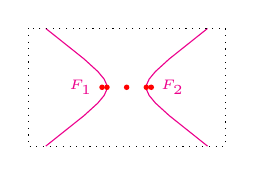
\begin{tikzpicture}[x=.25cm,y=.25cm,every node/.style={font=\tiny,text=magenta}]
		\coordinate(X')at(-5,0);
		\coordinate(X)at(5,0);
		\coordinate(Y')at(0,-3);
		\coordinate(Y)at(0,3);
		\coordinate(I)at(0,0);
		\coordinate(V1)at(-1,0);
		\coordinate(V2)at(1,0);
		\coordinate(F1)at(-1.25,0);
		\coordinate(F2)at(1.25,0);
		\draw[magenta]plot[samples=10,domain=-0.78:0.78]({1.*(1+(\x)^2)/(1-(\x)^2)},{0.75*2*(\x)/(1-(\x)^2)});
		\draw[magenta]plot[samples=10,domain=-0.78:0.78]({1.*(1+(\x)^2)/(-1+(\x)^2)},{0.75*2*(\x)/(-1+(\x)^2)});
		\foreach\p in{I,V1,V2,F1,F2}{\fill[red](\p)circle(1pt);}
		\node[left]at(F1){$ F_1 $};
		\node[right]at(F2){$ F_2 $};
		\draw[dotted](X'|-Y)--(X'|-Y')--(Y'-|X)--(Y-|X)--cycle;
		\end{tikzpicture}
		\subcaption{$ e=1.25 $}
	\end{subfigure}
	\begin{subfigure}[b]{.24\textwidth}
		\centering
		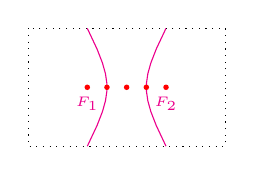
\begin{tikzpicture}[x=.25cm,y=.25cm,every node/.style={font=\tiny,text=magenta}]
		\coordinate(X')at(-5,0);
		\coordinate(X)at(5,0);
		\coordinate(Y')at(0,-3);
		\coordinate(Y)at(0,3);
		\coordinate(I)at(0,0);
		\coordinate(V1)at(-1,0);
		\coordinate(V2)at(1,0);
		\coordinate(F1)at(-2,0);
		\coordinate(F2)at(2,0);
		\draw[magenta]plot[samples=10,domain=-0.577:0.577]({1.*(1+(\x)^2)/(1-(\x)^2)},{1.73*2*(\x)/(1-(\x)^2)});
		\draw[magenta]plot[samples=10,domain=-0.577:0.577]({1.*(1+(\x)^2)/(-1+(\x)^2)},{1.73*2*(\x)/(-1+(\x)^2)});
		\foreach\p in{I,V1,V2,F1,F2}{\fill[red](\p)circle(1pt);}
		\node[below]at(F1){$ F_1 $};
		\node[below]at(F2){$ F_2 $};
		\draw[dotted](X'|-Y)--(X'|-Y')--(Y'-|X)--(Y-|X)--cycle;
		\end{tikzpicture}
		\subcaption{$ e=2 $}
	\end{subfigure}
	\begin{subfigure}[b]{.24\textwidth}
		\centering
		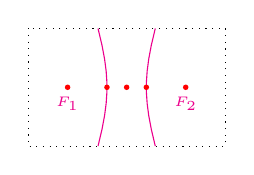
\begin{tikzpicture}[x=.25cm,y=.25cm,every node/.style={font=\tiny,text=magenta}]
		\coordinate(X')at(-5,0);
		\coordinate(X)at(5,0);
		\coordinate(Y')at(0,-3);
		\coordinate(Y)at(0,3);
		\coordinate(I)at(0,0);
		\coordinate(V1)at(-1,0);
		\coordinate(V2)at(1,0);
		\coordinate(F1)at(-3,0);
		\coordinate(F2)at(3,0);
		\draw[magenta]plot[samples=10,domain=-0.43:0.43]({1.*(1+(\x)^2)/(1-(\x)^2)},{2.83*2*(\x)/(1-(\x)^2)});
		\draw[magenta]plot[samples=10,domain=-0.43:0.43]({1.*(1+(\x)^2)/(-1+(\x)^2)},{2.83*2*(\x)/(-1+(\x)^2)});
		\foreach\p in{I,V1,V2,F1,F2}{\fill[red](\p)circle(1pt);}
		\node[below]at(F1){$ F_1 $};
		\node[below]at(F2){$ F_2 $};
		\draw[dotted](X'|-Y)--(X'|-Y')--(Y'-|X)--(Y-|X)--cycle;
		\end{tikzpicture}
		\subcaption{$ e=3 $}
	\end{subfigure}
	\begin{subfigure}[b]{.24\textwidth}
		\centering
		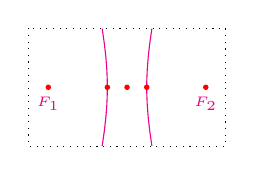
\begin{tikzpicture}[x=.25cm,y=.25cm,every node/.style={font=\tiny,text=magenta}]
		\coordinate(X')at(-5,0);
		\coordinate(X)at(5,0);
		\coordinate(Y')at(0,-3);
		\coordinate(Y)at(0,3);
		\coordinate(I)at(0,0);
		\coordinate(V1)at(-1,0);
		\coordinate(V2)at(1,0);
		\coordinate(F1)at(-4,0);
		\coordinate(F2)at(4,0);
		\draw[magenta]plot[samples=10,domain=-0.34:0.34]({1.*(1+(\x)^2)/(1-(\x)^2)},{3.87*2*(\x)/(1-(\x)^2)});
		\draw[magenta]plot[samples=10,domain=-0.34:0.34]({1.*(1+(\x)^2)/(-1+(\x)^2)},{3.87*2*(\x)/(-1+(\x)^2)});
		\foreach\p in{I,V1,V2,F1,F2}{\fill[red](\p)circle(1pt);}
		\node[below]at(F1){$ F_1 $};
		\node[below]at(F2){$ F_2 $};
		\draw[dotted](X'|-Y)--(X'|-Y')--(Y'-|X)--(Y-|X)--cycle;
		\end{tikzpicture}
		\subcaption{$ e=4 $}
	\end{subfigure}
\end{figure}
%
\begin{proposition*}
	អ៊ីពែបូលពីរដូចគ្នាកាលណាវាមានអ៊ិចសង់ទ្រីស៊ីតេ​ $ e $ ស្មើគ្នា។\\ ជាពិសេស អ៊ីពែបូលពីរប៉ុនគ្នាកាលណាវាដូចគ្នាហើយមានតម្លៃ $ a $ ឬ $ b $ ឬ $ c $ ស្មើគ្នា។
\end{proposition*}
%
\section{លក្ខណៈអុបទិចនៃអ៊ីពែបូល}
%
\begin{proposition*}
	កាំពន្លឺបាញ់ចេញពីកំណុំ $ F_1 $ ទៅចំណុច $ Q $ នៅលើផ្នែកម្ខាងទៀតនៃអ៊ីពែបូល ផ្លាតចេញតាមទិសនៃបន្ទាត់ $ (F_2Q) $~។
\end{proposition*}
%
\begin{figure}[H]
	\centering
	\caption{លក្ខណៈអុបទិកនៃអ៊ីពែបូល}
	\begin{tikzpicture}[x=.7cm,y=.7cm,every node/.style={font=\scriptsize,text=magenta}]
	\coordinate(O)at(0,0);
	\coordinate(X')at(-5,0);
	\coordinate(X)at(5,0);
	\coordinate(Y')at(0,-4);
	\coordinate(Y)at(0,4);
	\coordinate(I)at(0,0);
	\coordinate(F1)at(-2.97,0);
	\coordinate(F2)at(2.97,0);
	\coordinate(V1)at(-2,0);
	\coordinate(V2)at(2,0);
	\coordinate(Q)at(2.7,2);
	\coordinate(R)at(.8,1.33);
	\coordinate(S)at(1.77,0.47);
	\coordinate(T1)at(-.97,-4);
	\coordinate(T2)at(3.93,4);
	\coordinate(L1)at(-5,-.71);
	\coordinate(L2)at(5,2.81);
	\coordinate(M1)at(3.51,-4);
	\coordinate(M2)at(2.43,4);
	%x² / a² - y² / b² = 1; a=2, b=2.2
	\draw[magenta]plot[samples=25,domain=-0.59:0.59]({2.*(1+(\x)^2)/(1-(\x)^2)},{2.2*2*(\x)/(1-(\x)^2)});
	\draw[magenta]plot[samples=25,domain=-0.59:0.59]({2.*(1+(\x)^2)/(-1+(\x)^2)},{2.2*2*(\x)/(-1+(\x)^2)});
	\draw[dashed](X')--(X);
	\draw[violet](T1)--node[sloped,very near start,above]{$ (T) $}(T2);
	\draw[violet,dashed](L1)--(L2);
	\draw[violet,dashed](M1)--(M2);
	\draw[->](F1)--(Q);
	\draw[->](Q)--(M2);
	\pic[draw,angle radius=.7cm,angle eccentricity=1.25,"$ \alpha $"]{angle=T2--Q--M2};
	\pic[draw,angle radius=.7cm,angle eccentricity=1.25,"$ \alpha $"]{angle=F1--Q--T1};
	\foreach\p in{F1,F2,Q}{\fill[red](\p)circle(1.5pt);}
	\node[above]at(F1){$ F_1 $};
	\node[above right]at(F2){$ F_2 $};
	\node[above left]at(Q){$ Q $};
	\end{tikzpicture}
\end{figure}
%
\begin{answer}
	តាង $ Q $ ជាចំណុចមួយនៅលើអ៊ីពែបូលដែលមានកំណុំ $ F_1 $ និង $ F_2 $ ផ្សេងពីកំពូល~។ តាង $ (T) $ ជាបន្ទាត់ពុះនៃមុំ $ \angle F_1QF_2 $~។ តាង $ R $ ជាចំណុចនៅលើអង្កត់ $ [F_1Q] $ ដែល $ F_1R=2a $ និង $ S $ ជាចំណុចមួយនៅលើបន្ទាត់ $ (T) $ ផ្សេងពីចំណុច $ Q $~។ យើងនឹងបង្ហាញថា $ (T) $ ជាបន្ទាត់ប៉ះអ៊ីពែបូលត្រង់ $ Q $ គឺយើងបង្ហាញថា $ S $ មិននៅលើអ៊ីពែបូល។
	\begin{figure}[H]
		\centering
		\begin{tikzpicture}[x=.7cm,y=.7cm,every node/.style={font=\scriptsize,text=magenta}]
		\coordinate(O)at(0,0);
		\coordinate(X')at(-5,0);
		\coordinate(X)at(5,0);
		\coordinate(Y')at(0,-4);
		\coordinate(Y)at(0,4);
		\coordinate(I)at(0,0);
		\coordinate(F1)at(-2.97,0);
		\coordinate(F2)at(2.97,0);
		\coordinate(V1)at(-2,0);
		\coordinate(V2)at(2,0);
		\coordinate(Q)at(2.7,2);
		\coordinate(R)at(.8,1.33);
		\coordinate(S)at(1.77,0.47);
		\coordinate(T1)at(-.97,-4);
		\coordinate(T2)at(3.93,4);
		\coordinate(L1)at(-5,-.71);
		\coordinate(L2)at(5,2.81);
		\coordinate(M1)at(3.51,-4);
		\coordinate(M2)at(2.43,4);
		%x² / a² - y² / b² = 1; a=2, b=2.2
		\draw[magenta]plot[samples=25,domain=-0.59:0.59]({2.*(1+(\x)^2)/(1-(\x)^2)},{2.2*2*(\x)/(1-(\x)^2)});
		\draw[magenta]plot[samples=25,domain=-0.59:0.59]({2.*(1+(\x)^2)/(-1+(\x)^2)},{2.2*2*(\x)/(-1+(\x)^2)});
		\draw[dashed](X')--(X);
		\draw[violet](T1)--node[sloped,very near start,above]{$ (T) $}(T2);
		\draw[violet](L1)--(L2);
		\draw[violet](M1)--(M2);
		\draw(F1)--(S)--(F2);
		\draw(R)--(S);
		\pic[draw,angle radius=.7cm,angle eccentricity=1.25,"$ \alpha $"]{angle=T2--Q--M2};
		\pic[draw,angle radius=.7cm,angle eccentricity=1.25,"$ \alpha $"]{angle=F1--Q--T1};
		\pic[draw,angle radius=.7cm,angle eccentricity=1.25,"$ \alpha $"]{angle=T1--Q--M1};
		\foreach\p in{F1,F2,Q,R,S}{\fill[red](\p)circle(1.5pt);}
		\node[above]at(F1){$ F_1 $};
		\node[above right]at(F2){$ F_2 $};
		\node[above left]at(Q){$ Q $};
		\node[above]at(R){$ R $};
		\node[below]at(S){$ S $};
		\path(F1)--node[sloped,above]{$ 2a $}(R);
		\end{tikzpicture}
	\end{figure}
	ចំណុច $ Q $ នៅលើអ៊ីពែបូលនោះ $ F_1Q-QF_2=2a $ នាំឲ្យ $ QF_2=F_1Q-2a $~។
	ដោយ $ QR=F_1Q-F_1R=F_1Q-2a $ នោះយើងបាន $ QF_2=QR $~។ ត្រីកោណ $ \triangle QRS\cong\triangle QF_2S $ ព្រោះត្រីកោណទាំងពីរមាន
	\begin{itemize}
		\item ជ្រុង $ QS $ ជាជ្រុងរួម
		\item ជ្រុង $ QF_2=QR $ មូលហេតុខាងលើ
		\item មុំ $ \angle RQS=\angle F_2QS $ ព្រោះ $ (QS) $ ជាបន្ទាត់ពុះមុំ $ \angle RQF_2 $
	\end{itemize}
	វិបាក៖ $ RS=SF_2 $~។ អនុវត្តន៍វិសមភាពត្រីកោណក្នុង $ \triangle F_1RS $ យើងបាន
	\begin{equation*}
		F_1S<F_1R+RS\Rightarrow F_1S<2a+SF_2\;\text{ឬ}\; F_1S-SF_2<2a
	\end{equation*}
	មានន័យថា $ S $ មិននៅលើអ៊ីពែបូលទេ។
\end{answer}
%
\section{លំហាត់អ៊ីពែបូល}
%
\begin{enumerate}
	\item តើអ័ក្សទទឹងនៃអ៊ីពែបូល $ (H) $ ស្របអ័ក្សអាប់ស៊ីស ឬ ស្របអ័ក្សអរដោនេ?
	\begin{enumerate}[2]
		\item $ (H): \dfrac{(x-2)^2}{2^2}-\dfrac{(y-1)^2}{3^2}=1 $
		\item $ (H): \dfrac{(x-1)^2}{4^2}-\dfrac{(y+3)^2}{3^2}=1 $
		\item $ (H): \dfrac{(y+2)^2}{5^2}-\dfrac{(x+2)^2}{7^2}=1 $
		\item $ (H): \dfrac{(x-3)^2}{6^2}-\dfrac{(y+2)^2}{5^2}=1 $
		\item $ (H): \dfrac{(y-1)^2}{8^2}-\dfrac{(x-3)^2}{5^2}=1 $
		\item $ (H): \dfrac{(y-3)^2}{7^2}-\dfrac{(x+1)^2}{9^2}=1 $
	\end{enumerate}
	%
	\item សរសេរសមីការស្តង់ដានៃអ៊ីពែបូល $ (H) $ ខាងក្រោម៖
	\begin{enumerate}
		\item $ (H):16 x^2-32 x-9 y^2+36 y-164=0 $
		\item $ (H):-9 x^2-36 x+16 y^2+32 y-164=0 $
		\item $ (H):16 x^2+32 x-25 y^2+50 y-409=0 $
		\item $ (H):-25 x^2+100 x+4 y^2+24 y-164=0 $
		\item $ (H):-x^2-4 x+36 y^2+288 y+536=0 $
		\item $ (H):36 x^2+144 x-49 y^2+98 y-1669=0 $
	\end{enumerate}
	%
	\item សរសេរសមីការស្តង់ដានៃអ៊ីពែបូល $ (H) $ ដែលមាន
	\begin{enumerate}
		\item ផ្ចិត $ (0,0) $ កំពូល $ (0,3) $ និងកំណុំ $ (0,5) $
		\item ផ្ចិត $ (0,0) $ កំពូល $ (4,0) $ និងកំណុំ $ (5,0) $
		\item ផ្ចិត $ (1,2) $ កំពូល $ (4,2) $ និងកំណុំ $ (6,2) $
		\item ផ្ចិត $ (3,2) $ កំពូល $ (3,5) $ និងកំណុំ $ (3,7) $
		\item ផ្ចិត $ (-2,3) $ កំពូល $ (1,3) $ និងកំណុំ $ (-7,3) $
		\item ផ្ចិត $ (2,0) $ កំពូល $ (2,4) $ និងកំណុំ $ (2,-5) $
	\end{enumerate}
	%
	\item សរសេរសមីការស្តង់ដានៃអ៊ីពែបូល $ (H) $ ដែលមាន
	\begin{enumerate}
		\item កំពូល $ V_1(0,-4), V_2(0,4) $ និងកំណុំ $ (0,-5) $
		\item កំពូល $ V_1(-3,0), V_2(3,0) $ និងកំណុំ $ (5,0) $
		\item កំពូល $ V_1(2,2), V_2(4,2) $ និងកំណុំ $ (6,2) $
		\item កំពូល $ V_1(1,3), V_2(1,5) $ និងកំណុំ $ (1,-5) $
		\item កំពូល $ V_1(0,-2), V_2(4,-2) $ និងកំណុំ $ (7,-2) $
		\item កំពូល $ V_1(2,0), V_2(2,5) $ និងកំណុំ $ (2,-7) $
	\end{enumerate}
	%
	\item សរសេរសមីការស្តង់ដានៃអ៊ីពែបូល $ (H) $ ដែលមាន
	\begin{enumerate}
		\item កំណុំ $ F_1(0,-13), F_2(0,13) $ និងកំពូល $ (0,12) $
		\item កំណុំ $ F_1(-13,0), F_2(13,0) $ និងកំពូល $ (5,0) $
		\item កំណុំ $ F_1(12,2), F_2(2,2) $ និងកំពូល $ (10,2) $
		\item កំណុំ $ F_1(-1,-3), F_2(-1,7) $ និងកំពូល $ (-1,-1) $
		\item កំណុំ $ F_1(-5,2), F_2(4,2) $ និងកំពូល $ (0,2) $
		\item កំណុំ $ F_1(3,-3), F_2(3,6) $ និងកំពូល $ (3,3) $
	\end{enumerate}
	%
	\item សរសេរសមីការស្តង់ដានៃអ៊ីពែបូល $ (H) $ ដែលមាន
	\begin{enumerate}
		\item ផ្ចិត $ (0,0) $ កំពូល $ (3,0) $ និងអ៊ិចសង់ទ្រីស៊ីតេ $ e=\dfrac{5}{3} $
		\item ផ្ចិត $ (0,0) $ កំពូល $ (0,4) $ និងអ៊ិចសង់ទ្រីស៊ីតេ $ e=\dfrac{5}{4} $
		\item ផ្ចិត $ (1,2) $ កំពូល $ (1,4) $ និងអ៊ិចសង់ទ្រីស៊ីតេ $ e=\dfrac{5}{3} $
		\item ផ្ចិត $ (-2,1) $ កំពូល $ (3,1) $ និងអ៊ិចសង់ទ្រីស៊ីតេ $ e=\dfrac{13}{5} $
		\item ផ្ចិត $ (-3,-2) $ កំពូល $ (3,-2) $ និងអ៊ិចសង់ទ្រីស៊ីតេ $ e=2 $
		\item ផ្ចិត $ (0,2) $ កំពូល $ (0,5) $ និងអ៊ិចសង់ទ្រីស៊ីតេ $ e=3 $
	\end{enumerate}
	%
	\item សរសេរសមីការស្តង់ដានៃអ៊ីពែបូល $ (H) $ ដែលមាន
	\begin{enumerate}
		\item ផ្ចិត $ (0,0) $ កំណុំ $ (5,0) $ និងអ៊ិចសង់ទ្រីស៊ីតេ $ e=\dfrac{5}{3} $
		\item ផ្ចិត $ (0,0) $ កំណុំ $ (0,-5) $ និងអ៊ិចសង់ទ្រីស៊ីតេ $ e=\dfrac{5}{4} $
		\item ផ្ចិត $ (0,2) $ កំណុំ $ (13,2) $ និងអ៊ិចសង់ទ្រីស៊ីតេ $ e=\dfrac{13}{12} $
		\item ផ្ចិត $ (2,-3) $ កំណុំ $ (2,10) $ និងអ៊ិចសង់ទ្រីស៊ីតេ $ e=\dfrac{13}{5} $
		\item ផ្ចិត $ (-2,1) $ កំណុំ $ (8,1) $ និងអ៊ិចសង់ទ្រីស៊ីតេ $ e=\dfrac{5}{4} $
		\item ផ្ចិត $ (-3,-4) $ កំណុំ $ (-3,6) $ និងអ៊ិចសង់ទ្រីស៊ីតេ $ e=\dfrac{5}{3} $
	\end{enumerate}
	%
	\item សរសេរសមីការស្តង់ដានៃអ៊ីពែបូល $ (H) $ ដែលមាន
	\begin{enumerate}
		\item កំពូល $ V_1(0,-4),V_2(0,4) $ និងអាស៊ីមតូត $ y=\dfrac{4}{3}x,y=-\dfrac{4}{3}x $
		\item កំពូល $ V_1(1,-4),V_2(1,8) $ និងអាស៊ីមតូត $ y=\dfrac{3}{4}x+\dfrac{5}{4},y=-\dfrac{3}{4}x+\dfrac{11}{4} $
		\item កំពូល $ V_1(-7,-4),V_2(3,-4) $ និងអាស៊ីមតូត\\ $ 12x+5y+44=0,12x-5y+4=0 $
		\item កំពូល $ V_1(-10,-3),V_2(14,-3) $ និងអាស៊ីមតូត\\ $ 5x+12y+26=0,5x-12y-46=0 $
		\item កំពូល $ V_1(-8,-4),V_2(10,-4) $ និងអាស៊ីមតូត\\ $ -4x+3y=-16,-4x-3y=8 $
		\item កំពូល $ V_1(2,3),V_2(2,9) $ និងអាស៊ីមតូត $ y=x+4,y=-x+8 $
	\end{enumerate}
	%
	\item សរសេរសមីការស្តង់ដានៃអ៊ីពែបូល $ (H) $ ដែលមាន
	\begin{enumerate}
		\item កំណុំ $ F_1(-5,0),F_2(5,0) $ និងអាស៊ីមតូត $ y=\dfrac{3}{4}x,y=-\dfrac{3}{4}x $
		\item កំណុំ $ F_1(0,-10),F_2(0,10) $ និងអាស៊ីមតូត $ y=\dfrac{3}{4}x,y=-\dfrac{3}{4}x $
		\item កំណុំ $ F_1(7,-13),F_2(7,13) $ និងអាស៊ីមតូត $ 12x+5y=84,12x-5y=84 $
		\item កំណុំ $ F_1(-13,3),F_2(7,3) $ និងអាស៊ីមតូត $ 4x+3y+3=0, 4x-3y+21=0 $
		\item កំណុំ $ F_1(4,6),F_2(4,-14) $ និងអាស៊ីមតូត $ 4x-3y-28=0 $%4x+3y+4=0,
		\item កំណុំ $ F_1(-28,-3),F_2(24,-3) $ និងអាស៊ីមតូត $ 5x+12y+46=0 $%,5x-12y+26=0
	\end{enumerate}
	%
	\item រកកូអរដោនេផ្ចិត កំពូល កំណុំ និងសមីការអាស៊ីមតូតនៃអ៊ីពែបូល $ (H) $
	\begin{enumerate}[2]
		\item $ (H):\dfrac{(x-0)^2}{3^2}-\dfrac{(y-0)^2}{4^2}=1 $
		\item $ (H):\dfrac{(y-0)^2}{3^2}-\dfrac{(x-0)^2}{4^2}=1 $
		\item $ (H):\dfrac{(x-1)^2}{5^2}-\dfrac{(y-2)^2}{12^2}=1 $
		\item $ (H):\dfrac{(x-2)^2}{6^2}-\dfrac{(y+3)^2}{8^2}=1 $
		\item $ (H):\dfrac{(y+2)^2}{8^2}-\dfrac{(x-1)^2}{6^2}=1 $
		\item $ (H):\dfrac{(x+3)^2}{12^2}-\dfrac{(y+3)^2}{5^2}=1 $
	\end{enumerate}
\end{enumerate}
%